\section{Separate Temporal Compression Pilot}
\label{sec:temporal-residual-validation}

This appendix records a separate exploratory redesign, not an extension of the
scalar method's test results. One new CIFAR-100N base (initialization42, fixed
split 42) completed 50 epochs, retaining end-of-epoch snapshots 1--5 before a separate frozen
clean-test evaluation. These snapshots supplied full class probabilities on
identical canonical training images. A residual MLP on the selected base's frozen
2048-dimensional features was fitted to their mean by KL divergence. Its hidden
width is 256, its output layer starts at zero, and it uses the original reserved
meta partitions. The deployed posterior is
$\operatorname{softmax}(\log p_{\mathrm{base}}+\alpha h(f(x)))$.
The head checkpoint minimizes reserved meta-validation KL; the fixed
$\alpha\in\{0,.25,.5,1\}$ grid uses noisy base-validation accuracy, then cross
entropy, then smaller $\alpha$. No policy was selected on clean test data.

\begin{table}[h]
\centering
\caption{Single-base noisy-validation pilot (5,000 observed labels). These are
not clean-test accuracies or significance estimates.}
\begin{tabular}{lrrr}
\toprule
Predictor & Accuracy (\%) & Gain (pp) & NLL\\
\midrule
Selected base(FP32) &54.66&0.00&1.916\\
Residual student &56.08&1.42&1.861\\
Five-snapshot mean &56.56&1.90&1.826\\
\bottomrule
\end{tabular}
\end{table}

Both selected interpolation strengths are 1. The base checkpoint is epoch 2
(one-based), and the residual checkpoint is epoch 4 of 25. Meta-validation KL
falls from 0.1249 at initialization to 0.06872, while later training continues to
reduce fitting KL without improving the selected validation minimum. The ratio
$1.42/1.90\approx.747$ describes retained noisy-validation gain on this split;
it is not a cross-dataset transfer guarantee. Reuse of noisy validation for
checkpoint and strength selection limits interpretation. The compact export
supports 35 consistency checks but contains neither binary weights nor per-image
probabilities, so no paired interval or raw replay is claimed.

This mechanism compresses a snapshot mean and is related to existing snapshot
distillation; no new temporal-attribution or novelty claim is established here.
The following subsection records independent-base follow-ups; matched
non-temporal ensemble controls remain outstanding. The main manuscript's scalar results are unchanged.

\begin{figure}[ht]
\centering
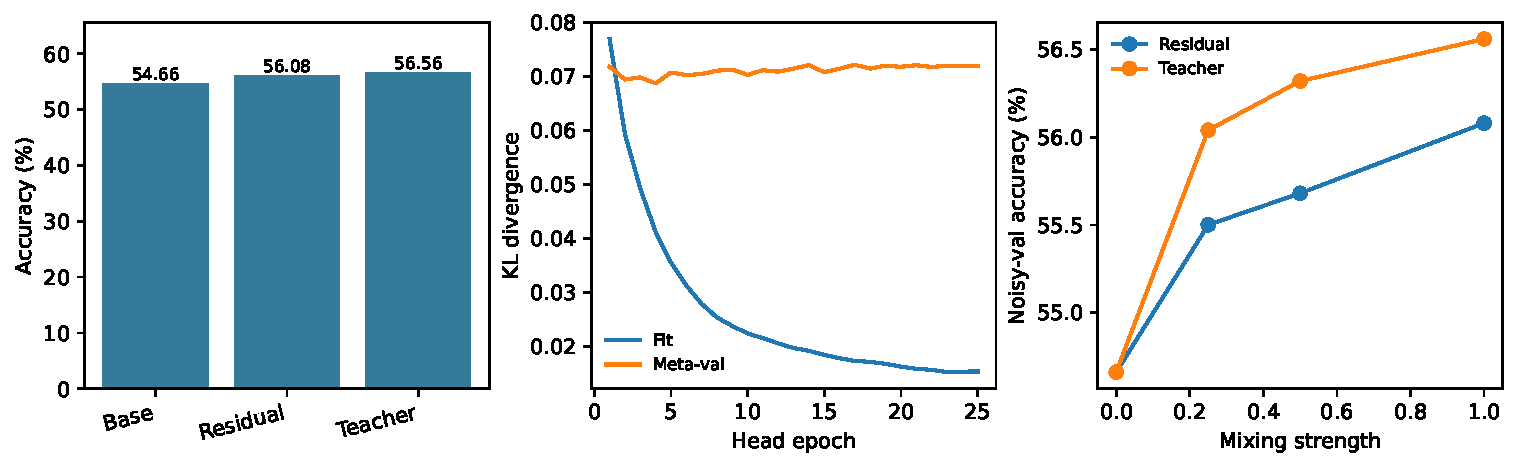
\includegraphics[width=\textwidth]{figures/temporal_residual_validation.pdf}
\caption{Validation-only pilot: selected accuracies, head fitting curves, and
the complete fixed strength grid. One base and one head initialization; no
test-result or significance interval is shown.}
\end{figure}

\subsection{Frozen Clean-Test Evaluation}

The already selected policy and checkpoint were evaluated without refitting or
changing either interpolation strength. Source, checkpoint, evidence-cache and
policy identities were checked before test access. Saved per-image probabilities
on all 10,000 official CIFAR-100 test images reproduce the exported metrics and
paired intervals; 46 local replay checks passed.

\begin{table}[ht]
\centering
\caption{Separate frozen pilot, one fitted base and head. ECE uses 15 bins.
The five-snapshot teacher requires five backbone passes; the student uses one
backbone pass plus its residual MLP.}
\begin{tabular}{lrrrr}
\toprule
Predictor & Accuracy (\%) & NLL & Brier & ECE\\
\midrule
Selected base &69.79&1.1273&.4373&.1226\\
Residual student &71.83&1.0867&.4198&.1498\\
Five-snapshot mean &73.15&1.0442&.4087&.1620\\
\bottomrule
\end{tabular}
\end{table}

Student minus base accuracy is $+2.04$ percentage points, with nominal paired
95\% bootstrap interval $[1.46,2.65]$. Teacher minus base is $+3.36$
$[2.70,4.04]$ points; student minus teacher is $-1.32$ $[-1.86,-0.77]$ points.
These 2,000-draw intervals condition on the fitted models and test examples;
they have no multiplicity adjustment and do not estimate between-base variation.
The student retains $2.04/3.36=60.7\%$ of the teacher's accuracy gain.
NLL and Brier improve, while ECE worsens; hence improved calibration is not
claimed. Student own-error AUROC is .8313 versus .8169 for the base, but these
scores target different error events. Against the fixed original-base error
event, student confidence gives AUROC .8355. These single-base results support
feasibility, not a demonstrated temporal-specific advantage or broad robustness.

\begin{figure}[ht]
\centering
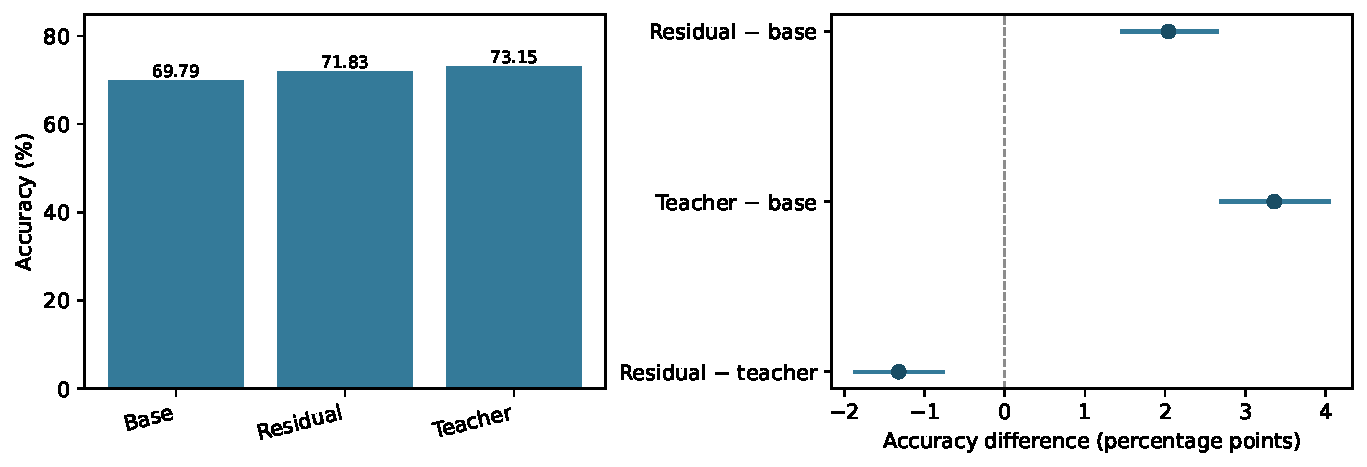
\includegraphics[width=\textwidth]{figures/temporal_residual_test.pdf}
\caption{Frozen clean-test accuracy and predeclared paired comparisons.
Intervals condition on one fitted base/head. No policy was selected on test.}
\end{figure}

\subsection{Independent-Base Follow-ups and Fixed Single-Epoch Control}

The follow-up protocol was specified after observing the seed42 pilot test,
not before that pilot. Independent base seeds43 and44 retain base split42,
the same 50-epoch training protocol and head seed42. Each base supports two
heads with identical features, meta partitions, initialization, optimizer,
25-epoch budget and validation selection: the mean of snapshots1--5, or the
single fixed epoch1 teacher. Both policies were frozen before either test was
accessed. Raw predictions reproduce all exported metrics and comparisons;
155 local checks passed. This control tests multiple-snapshot compression
against one fixed early snapshot, not an equal-compute independent ensemble.

\begin{table}[ht]
\centering
\caption{Clean-test accuracy (\%). Mean and sample SD describe three independent
base initializations with a fixed head seed and data split; SD is not a confidence
interval. The epoch1 control was run only for seeds43/44.}
\begin{tabular}{lrrrr}
\toprule
Base seed & Base & Temporal student & Five-snapshot mean & Epoch1 student\\
\midrule
42 &69.79&71.83&73.15&---\\
43 &69.98&71.45&73.55&71.13\\
44 &69.04&71.55&73.07&70.62\\
\midrule
Mean $\pm$ SD & $69.60\pm.50$ & $71.61\pm.20$ & $73.26\pm.26$ &---\\
\bottomrule
\end{tabular}
\end{table}

Student gains over the base are $+2.04$, $+1.47$ and $+2.51$ percentage points
(mean $+2.01$, sample SD $.52$). The later two conditional paired-example
intervals are $[1.06,1.88]$ and $[1.92,3.12]$ points. However, single-epoch
students also improve the base by $+1.15$ and $+1.58$ points. Temporal minus
single-epoch student is $+.32$ $[-.02,.68]$ points on seed43 and $+.93$
$[.43,1.45]$ points on seed44; the mean descriptive difference is $.625$ points.
The seed43 interval includes zero. These nominal intervals are unadjusted and
condition on the fitted models. Two control bases cannot establish robust
between-base superiority. ECE worsens relative to the base on all three seeds.
Thus compression gains replicate, but attributing all of the gain to temporal
history, or claiming improved calibration, is unsupported. Comparison against
stronger validation-selected single-snapshot and non-temporal ensemble controls
was pending at this stage; the S2 controls below address several of these gaps.
The strongest ensemble teacher still exceeds each student.

\begin{figure}[ht]
\centering
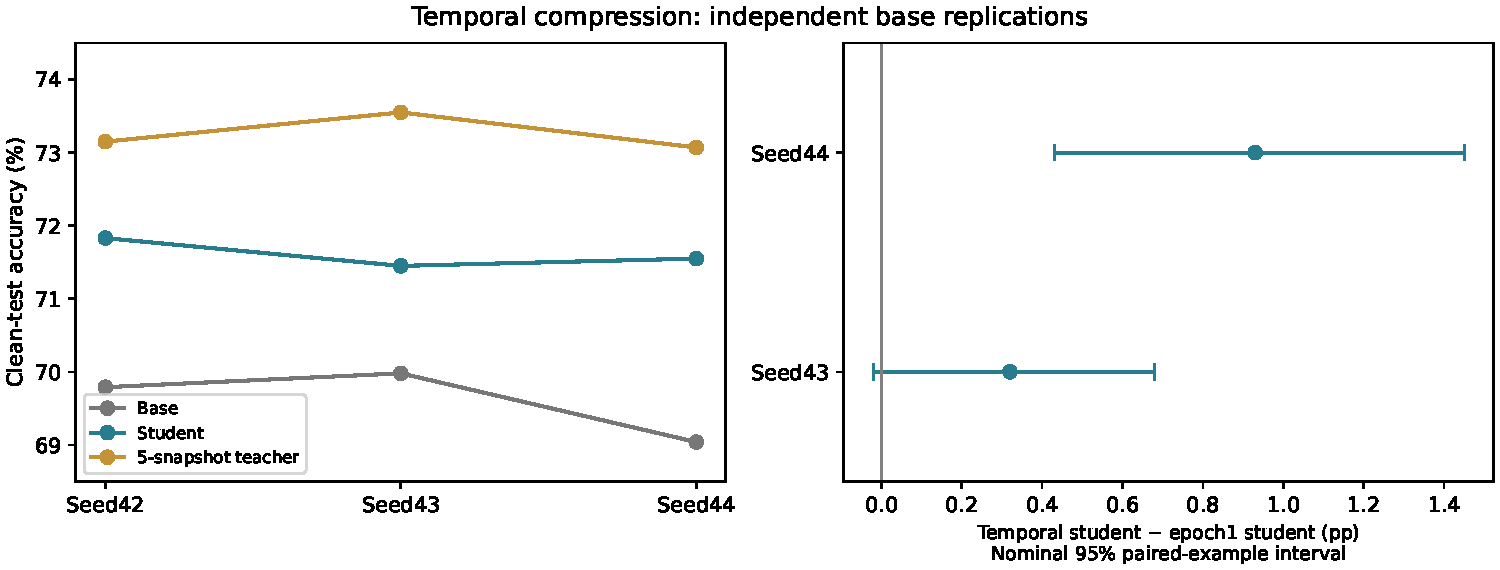
\includegraphics[width=\textwidth]{figures/temporal_residual_replications.pdf}
\caption{Independent base seeds and the fixed epoch1 head control.
Conditional intervals are not uncertainty across training runs.}
\end{figure}

\subsection{Exploratory Validation-Selected Single-Snapshot Control}

After the preceding test results were known, a stronger single-teacher control
was specified for base seeds43/44. Epochs1--5 and interpolation strengths
$\{0,.25,.5,1\}$ were ranked using noisy-validation accuracy, then lower NLL,
smaller strength and earlier epoch. The selected epochs are5 and3, respectively.
Identical residual heads and meta splits were used, with both control policies
frozen before their evaluation. Because the official test had already been
examined, this is explicitly post-pilot exploratory reuse, not independent
confirmatory evidence. Raw prediction replay passed81 checks.

\begin{table}[ht]
\centering
\caption{Validation-selected single-snapshot control. Accuracy in percent;
the two-pass interpolation uses the original base and selected teacher.}
\begin{tabular}{lrrrr}
\toprule
Seed & Base & Single student & Temporal student & Two-pass interpolation\\
\midrule
43&69.98&70.97&71.45&71.67\\
44&69.04&71.25&71.55&71.77\\
\bottomrule
\end{tabular}
\end{table}

Temporal minus selected-single student is $+.48$ points (nominal paired
95\% interval $[.10,.90]$) and $+.30$ points ($[-.17,.78]$). The descriptive
mean difference is $.39$ points across two bases, not a between-base significance
estimate. Substantial gains are therefore reproduced by single-snapshot
distillation, limiting attribution of the full base-relative improvement to
temporal aggregation. The simple two-pass interpolation is $.22$ points above
the temporal student on each base, although the conditional intervals for
this difference include zero. The latency of the one-pass student and the five-pass teacher was measured
separately on T4. The later CIFAR-10.1 evaluation did not confirm the
residual accuracy gain (Section~\ref{sec:confirmation-s4}).

\begin{figure}[ht]
\centering
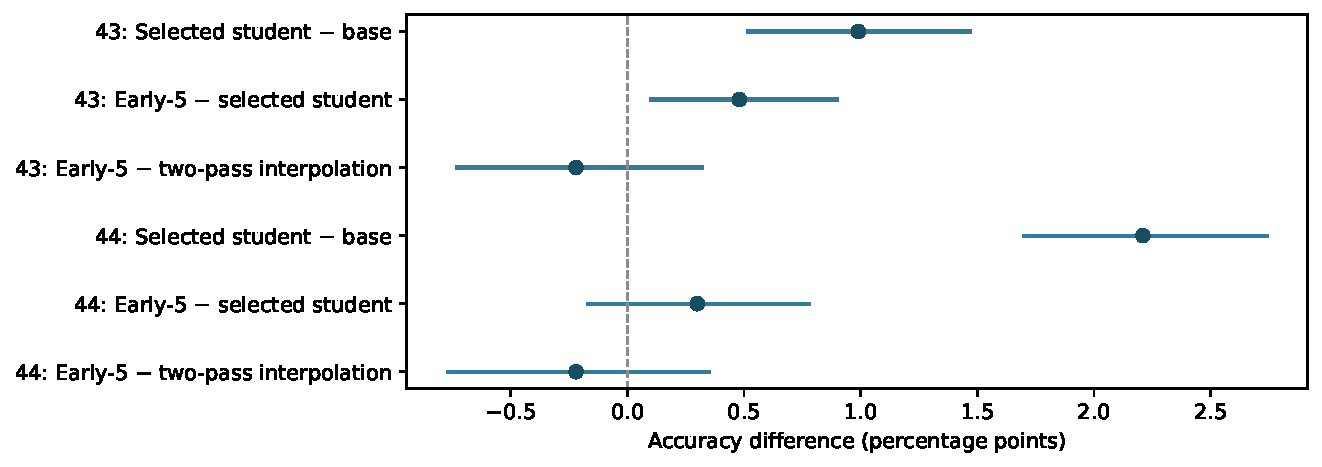
\includegraphics[width=\textwidth]{figures/temporal_selected_control.pdf}
\caption{Exploratory selected-single comparison. Two-pass interpolation is
reported separately from one-backbone-pass student heads.}
\end{figure}


\subsection{Exploratory S2 Post-Hoc Controls Across Three Bases}

Two frozen packages completed13 new heads:10 controls in A and three
independent-teacher students in B. The head seed remains42. All heads train on
noisy annotations or teacher probabilities; clean test labels are evaluation-only.
The direct soft-target head uses the same frozen features, Early-5 target and MLP
width as the residual head, without the base-log-probability offset during fitting;
both use validation-selected interpolation at inference. Early-2 averages states1
and5. Independent-2 averages the other two trained bases for each recipient.
Thus teacher pass counts match Early-2, but training costs do not: independent
teachers require additional base training and donors are shared between recipients.
The selected base checkpoint is epoch2 for all recipients, and states1--5 belong
to CE warmup. The contrasts cannot isolate a general causal effect of temporal
history from optimization phase or teacher quality.

\begin{table}[ht]
\centering
\caption{Exploratory CIFAR-100N controls: accuracy (\%). All student methods use one backbone pass. Means give equal weight to the three original bases; the head seed is fixed at42.}
\begin{tabular}{lrrrr}
\toprule
Method &42&43&44&Mean\\
\midrule
Base & 69.79 & 69.98 & 69.04 & 69.60\\
Selected single & 71.51 & 70.97 & 71.25 & 71.24\\
Noisy-label head & 71.13 & 71.45 & 70.84 & 71.14\\
Early-2 residual & 71.38 & 71.85 & 71.41 & 71.55\\
Early-5 residual & 71.83 & 71.45 & 71.55 & 71.61\\
Early-5 direct & 71.51 & 71.58 & 71.51 & 71.53\\
Independent-2 student & 71.95 & 71.81 & 71.84 & 71.87\\
\bottomrule
\end{tabular}
\end{table}


Early-5 exceeds the validation-selected single-snapshot student by .32, .48 and
.30 percentage points (mean .367). The nominal paired intervals include zero
for seeds42 and44. Its mean advantage over the direct soft-target head is only
.077 points; all three corresponding intervals include zero. Its mean advantage
over Early-2 is .063 points with mixed seed-wise signs. Independent-2 students
reach 71.87\% versus71.61\% for Early-5; shared donors and conditional intervals
preclude claiming independent, statistically established superiority. These
comparisons retain the base-relative compression gain while failing to establish
a distinctive benefit of the residual parametrization or five-state target.

Deterministic local replay of supplied raw predictions passed503 checks,
including source hashes, policy consistency, sample alignment, exported metrics
and paired comparisons. Cross-platform teacher interpolation matches within
$10^{-6}$ absolute and $2\times10^{-5}$ relative tolerance with exactly matching
class decisions; this is not bitwise reconstruction. Small exports omit fitted
weights and train/validation target arrays, so training and complete model-forward
regeneration were not performed locally. The seed42 full20-row epoch-selection
grid was subsequently recovered from original Kaggle Output version362957682.
Replaying its ranking exactly reproduces the frozen policy (epoch3, strength.5);
this closes the missing-grid gap without regenerating validation predictions.

Risk-coverage area was absent from the original S2 export. Supplemental local
analysis computes mean risk at discrete coverages with expected random ordering
inside exact confidence ties. Mean AURC is .11786 for the base, .10240 for Early-5,
.10394 for the direct head and .10197 for Independent-2. This tie-safe definition
is separate from historical risk-area exports. ECE remains worse for Early-5
than the base. GPU latency and end-to-end cost have not been measured; the
accuracy block does not complete the full S2 decision gate. All comparisons
reuse a previously examined test set and are exploratory.

\begin{figure}[ht]
\centering
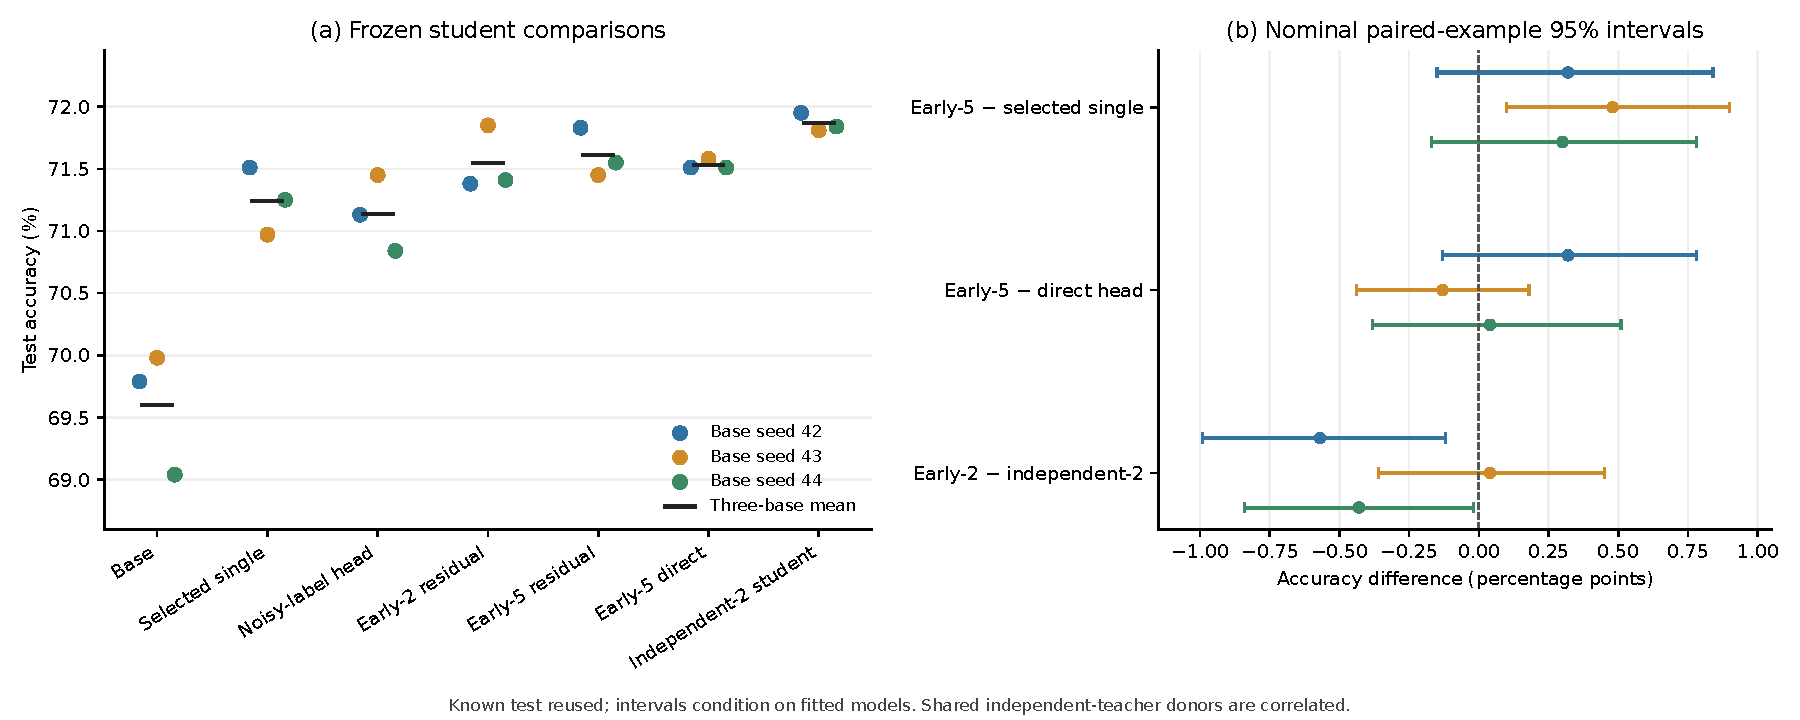
\includegraphics[width=\textwidth]{figures/posthoc_controls.pdf}
\caption{S2 frozen controls. Black marks are descriptive means over three bases.
Intervals condition on fitted models and do not quantify training-run uncertainty.}
\end{figure}
